\documentclass[12pt]{iopart}
\newcommand{\gguide}{{\it Preparing graphics for IOP Publishing journals}}

\usepackage{harvard}
\usepackage{graphicx}
\graphicspath{{./figures/}}

\usepackage[]{biblatex}
\addbibresource{cites.bib}

%Uncomment next line if AMS fonts required
%\usepackage{iopams}
\begin{document}

\section{Introduction}

Three-dimensional manufacturing is crucial for future devices in a broad size range for the fields of fluidics and photonics. Polymer materials are promising for these areas of application due to a broad spectrum of available polymers and emerging patterning technologies as well as the potential for efficient tuning of material properties. Reflowing lithographically prepatterned, binary polymer structures is an established method for microlens fabrication,
The surface dynamics of viscous polymer films have been widely studied for fundamental purposes, as well as for applications. Several experimental approaches, mainly based on scattering correlation methods onto isodense patterns, have been carried out. No studies have dealt simultaneously with both detailed theoretical aspects and corresponding nanoscale experiments.

By now, two different approaches to simulation of resist reflow exist. The first one, analytical, bases on 2D Navier-Stokes equation coupled to continuity equation with the assumption of no slip length and no Marangoni effect but considering Laplace pressure and Hamaker energy~\cite{Leveder_2010}. In this approach polymer surface is Fourier transformed and reflow process is simulated by decay of profile harmonics:

\begin{eqnarray}
	h(x, t) = h_0 + \tilde{h}(x, t),\\
	\tilde{h}(x, t) = \sum_{-\infty}^{+\infty} a_n(0) \exp \left(-\frac{t}{\tau_n}+i n \frac{2 \pi}{\lambda} x \right),\\
	\tau_n = \frac{3 \eta}{\gamma h_0^3} \times \left( \frac{\lambda}{2 \pi n} \right)^4.
\end{eqnarray}

where $\lambda$ -- profile period, $\eta$, $\gamma$ -- polymer viscosity and surface tension, respectively, $a_n(0)$ -- Fourier coefficients of initial polymer profile, $h_0$ -- polymer layer thickness. Polymer viscosity depends both on temperature and polymer molecular weight, which should be taken into account in simulation. Temperature dependence of viscosity could be described by Williams–Landel–Ferry (WLF) equation~\cite{bird1987dynamics_WLF}:
\begin{equation} \label{eq:WLF}
	\log \left( \frac{\eta(T)}{\eta(T_0)} \right) = -\frac{C_1(T-T_0)}{C_2+(T-T_0)},
\end{equation}
which parameters $\eta(T_0)$, $C_1$, $C_2$ and $T_0$ for three different resists could be found in Table~\ref{table:WLF}~\cite{aho2008measurement_WLF}.




The dependence of polymer viscosity on its molecular weight could be described by empirical formula:
\begin{equation} \label{eq:3p4_3p1}
	\eta \propto M_n^\alpha,
\end{equation}
where $M_n$ -- number average polymer molecular weight. For PMMA $\alpha$ comprises 3.4 at $M_n \geq 48 000$ and 1.4 at $M_n < 48 000$~\cite{Leveder_2010, Bueche_3p4_1p4}. Equations~(\ref{eq:WLF}, \ref{eq:3p4_3p1}) allows one to calculate polymer viscosity for different temperatures and molecular weights (Fig.~\ref{fig:eta_vary_T_Mn}).

The precision of this analytic approach is quite high for the simulation of polymer reflow when $a_n(t) \ll h_0$, however, it couldn't be applied in case of non-uniform polymer viscosity profile.


\begin{figure}[h]
	\begin{center}
		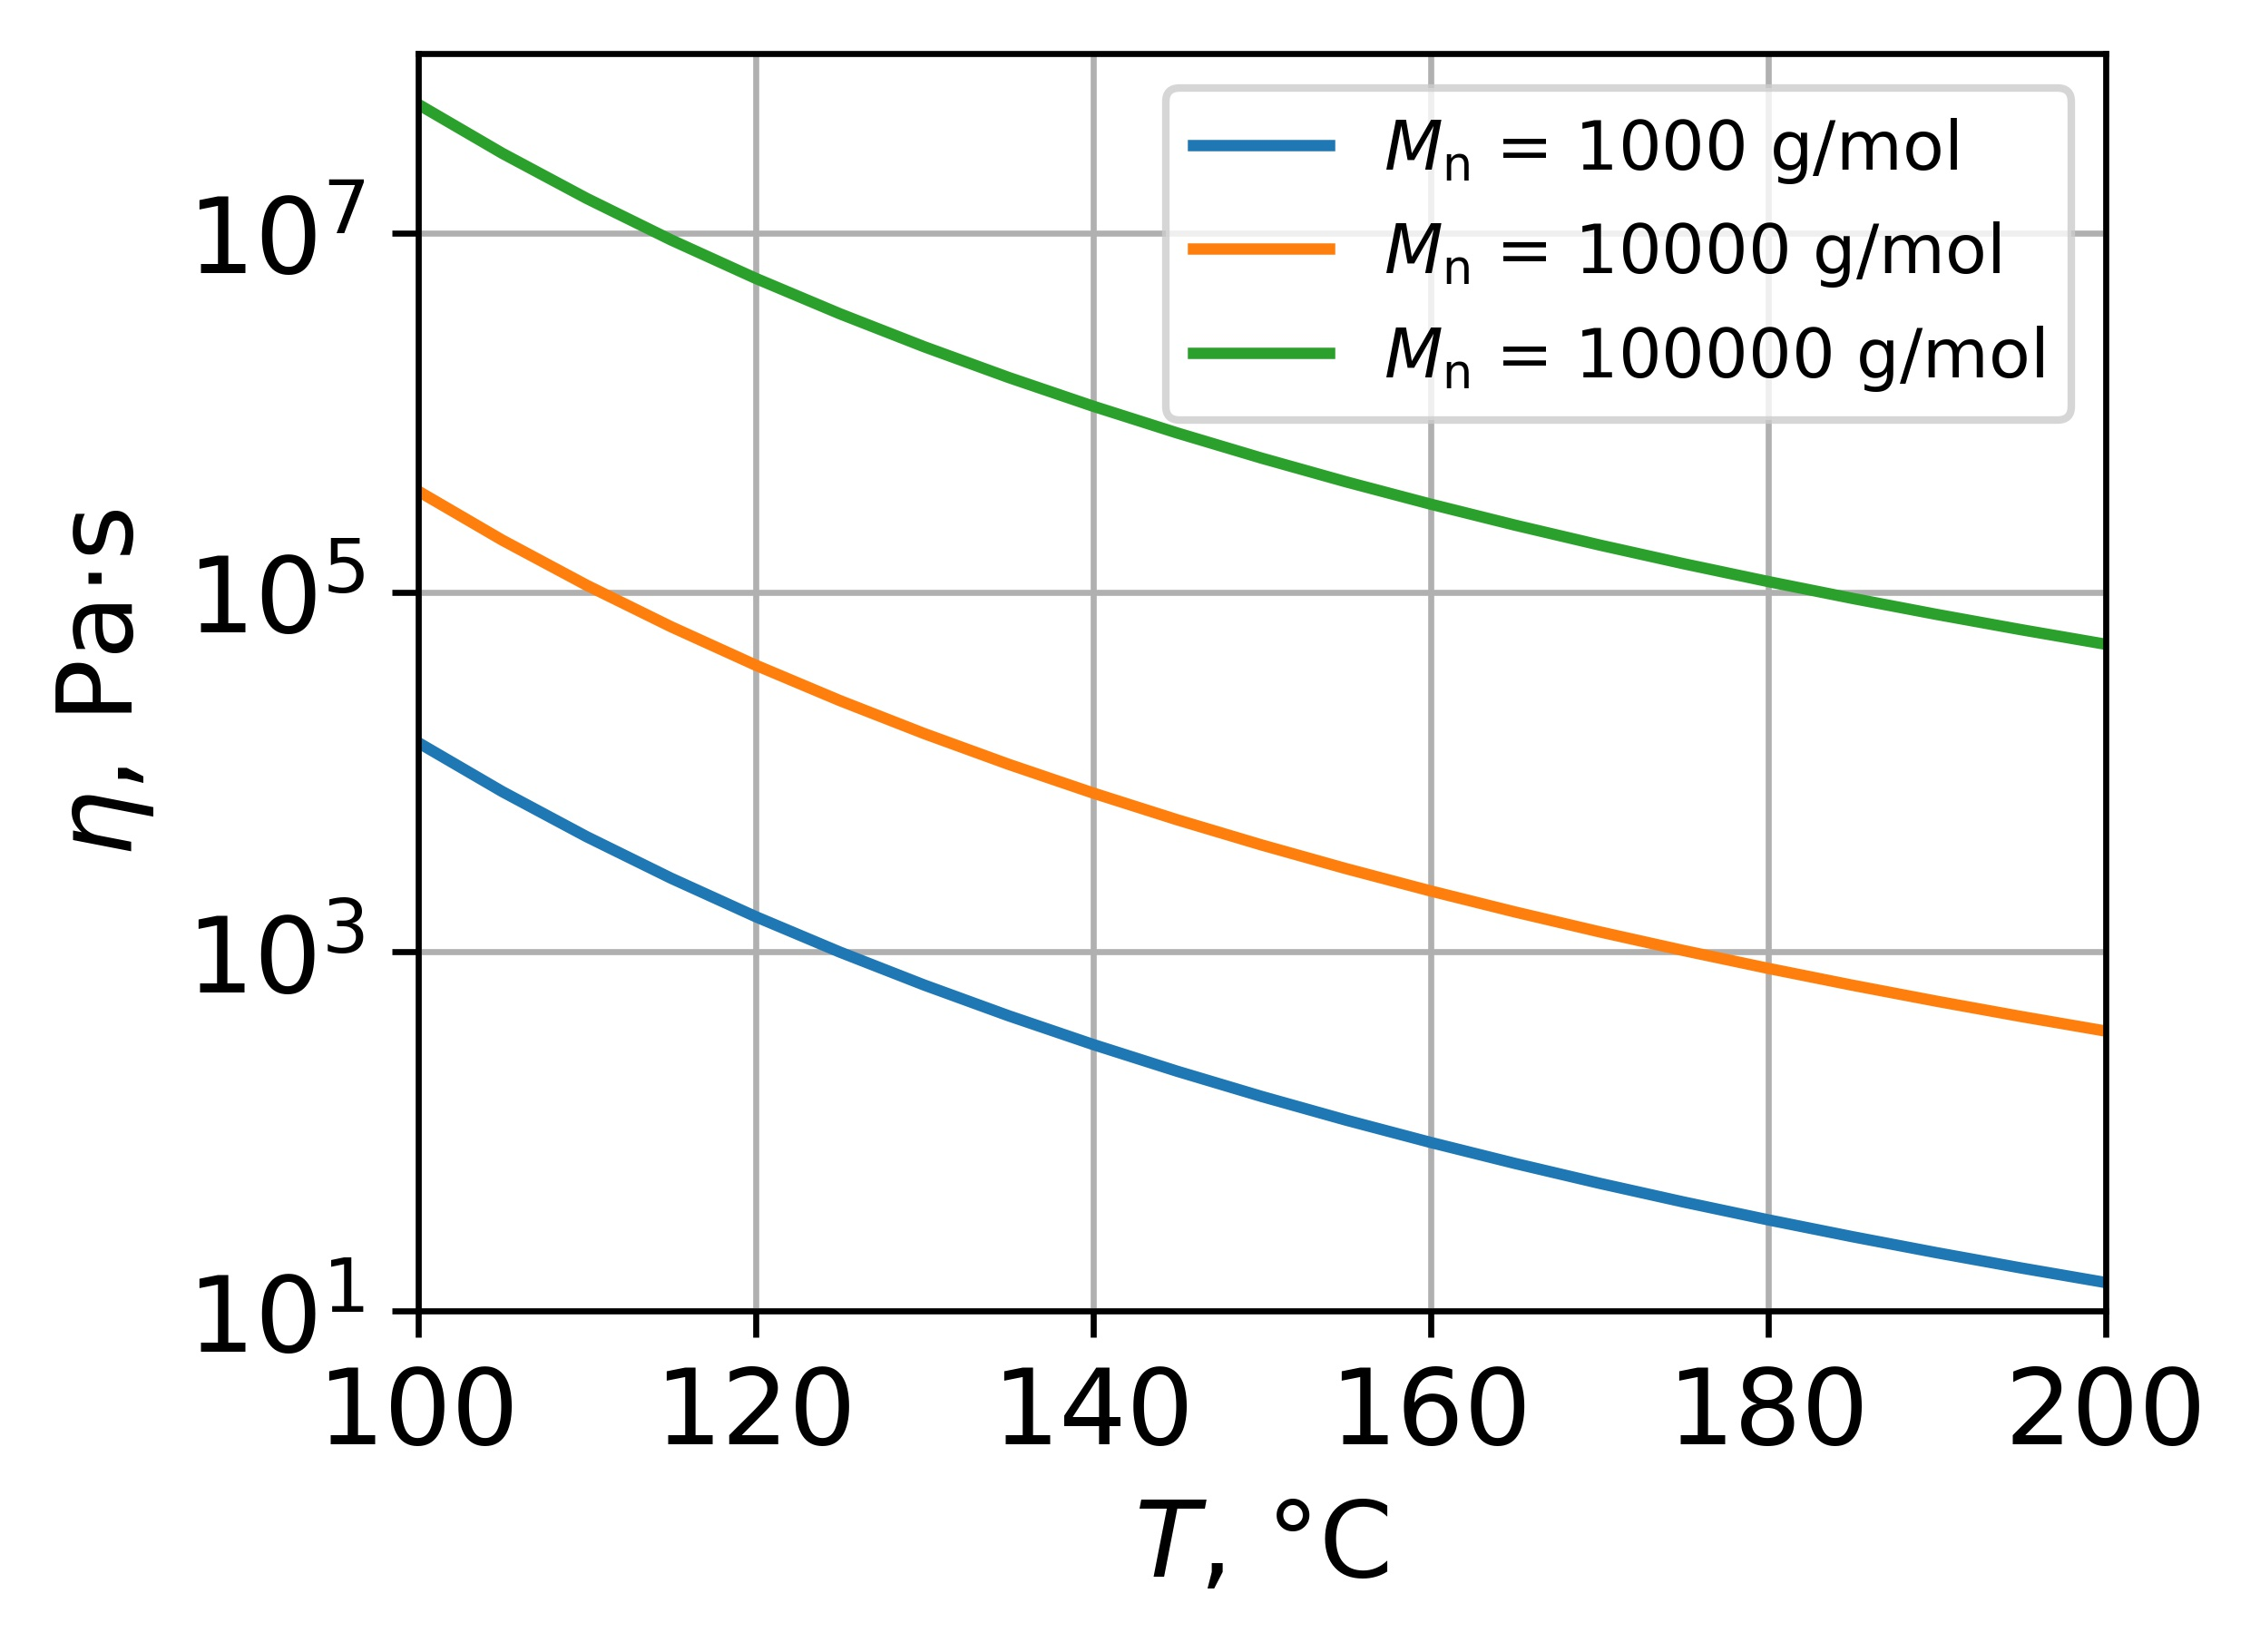
\includegraphics[width=0.6\linewidth]{eta_vary_T_Mn}
	\end{center}
	\vspace{-2em}
	\caption{Temperature PMMA viscosity dependencies in case of various number average molecular weight values, obtained by equations~(\ref{eq:WLF}, \ref{eq:3p4_3p1}).}
	\label{fig:eta_vary_T_Mn}
\end{figure}


The second approach, numerical one, is based on search of minimal surface by finite elements method. It is processed by software ``Surface Evolver'' (SE) -- program for the modelling of liquid surfaces shaped by various forces and constraints. In this approach polymer surface is divided into triangle facets defined by vertices $v_0$, $v_1$ and $v_2$ and oriented edges $\vec{e_0}$, $\vec{e_1}$ and $\vec{e_2}$, and the polymer reflow is simulated by moving of facet vertices. The force on vertex $v_0$ (beginning of oriented edge $\vec{e_0}$) is
\begin{equation}
	\vec{F}_{V_0}=\frac{\gamma_i}{2} \cdot \frac{\vec{e}_1 \times\left(\vec{e}_0 \times \vec{e}_1\right)}{\left\|\vec{e}_0 \times \vec{e}_1\right\|},
\end{equation}
where $\gamma_i$ -- is surface tension of $i$-th facet. For the most realistic simulation SE could be operated in the area normalization mode to approximate a vertex motion by mean curvature. In this mode, the velocity of a vertex is proportional to force and indirectly proportional to the area of the facets surrounding this vertex. The $i$-th facet has three vertices associated with it, therefore the relative area contribution to the force of one vertex is 1/3 the area of the surrounding facets $A$. The vertex velocity in the area normalization mode is
\begin{equation}
	\vec{v} = \frac{\vec{F}}{A/3} \cdot \mu,
\end{equation}
where $\mu$ is vertex mobility. The vector of vertex movement $\vec{\delta}$ is then calculated as product of vertex velocity and \textit{scale} factor $s$, the physical representation of time:
\begin{equation} \label{eq:SE_delta}
	\vec{\delta} = \vec{v} \cdot s.
\end{equation}


However, both approaches couldn't be applied in case of non-uniform polymer viscosity profile in general. This conditions could be achieved, for example, in case of e-beam exposed polymer reflow, which is used as a smoothing process for structures obtained by grayscale e-beam lithography. Despite Kirhner demonstrated the capability of Surface Evolver for the simulation of ``step structure'', it consisted in only two regions with different polymer molecular weight. Thus, existing methods seem to need modification for applicability to simulation on non-uniform resist reflow.


\section{Simulation of polymer viscosity distribution}
Simulation of polymer viscosity distribution during exposure was based on Monte-Carlo simulation of e-beam scattering in PMMA. The algorithm described in \cite{my_MEE} was used to simulate polymer main-chain scissions (Fig.~\ref{fig:sci_hist}).


Dividing line volume into 5nm cells allowed to simulate depolymerization chain initiation constant in each cell (the number of scissions per monomer per 1 s). This constant was used for simulation of PMMA local molecular weight using approach described in~\cite{Boyd_1, Boyd_2, Boyd_3}. It bases in the assumption of Schulz-Zimm polymer weight distribution~\cite{Schulz-Zimm_distribution}:
\begin{equation} \label{eq:Schulz-Zimm_distribution}
	P_n = C_0 n^z \exp (-n/y)
\end{equation}
where $P_n$ -- number of molecules with degree of polymerization equal to $n$, $C_0$ -- normalization factor. Parameter $z$ describes the width of distribution:
\begin{equation} \label{eq:Schulz-Zimm_1}
	M_w / M_N=(z+2) /(z+1),
\end{equation}
where $M_n$ and $M_w$ -- number average and weight average molecular weight, respectively, parameter $y$ is related to number average polymerization degree $x$:
\begin{equation} \label{eq:Schulz-Zimm_2}
	x=y(z+1).
\end{equation}

\noindent In this case polymer degradation could be described by equation on polymer molecular weight moments:
\begin{equation} \label{eq:moment_equation}
	\frac{d M_i}{d t}=k_s(\frac{2}{i+1}-1) M_{i+1}+\frac{d M_0}{d t}-k_s M_1 - \frac{i}{\gamma}(k_s M_i+\frac{d M_{i-1}}{d t}) \quad(i \geq 1),
\end{equation}
where $1/\gamma$ -- average depolymerization zip length, $M_i$ -- moment of molecular weight distribution on $i$-th order:
\begin{equation}
	M_i=\sum_{n=2}^{\infty} n^i P_n,
\end{equation}
$k_s$ -- depolymerization chain initiation constant. The result of PMMA molecular weight simulation for different exposure moments is shown in Fig.~\ref{fig:Mn_hist}

Average depolymerization zip length could be obtained by exponential fit of values provided by Mita~\cite{Mita_PMMA_zip_lengths_T} for PMMA in case of depolymerization termination or of chain transfer at the end of molecule (Fig.~\ref{fig:zip_lengths}).


\noindent Using the relation between $M_i$, $M_1$, $y$ and $z$:
\begin{equation}
	M_i=M_1 \prod_{n=2}^i(z+n) y^{i-1},
\end{equation}
one could describe Shulz-Zimm distribution parameter ($C_0$, $z$ and $y$) changes by three equations of the form of~(\ref{eq:moment_equation}) (see Appendix). This results in local $M_n$ and $M_w$ dependence on exposure time (Fig.~\ref{fig:Mn_Mw_tau}), which allow to calculate local polymer viscosity (Fig.~\ref{fig:Mn_hist}).


\section{Determination of polymer vertex mobility}
Obtained polymer local viscosity distribution still could not be utilized for reflow simulation -- the approach based on Fourier transform of profile requires uniform resist viscosity. On the other hand, the numerical approach bases on vertex mobilities, not viscosity. Therefore, one should introduce the correlation between polymer viscosity and vertex mobilities of its surface.

For this purpose, we simulated the reflow of rectangular PMMA gratings by both approaches. Grating parameters correspond to realistic values for NIL -- 2 $\mu$m pitch and 280 nm depth. The viscosity of PMMA varied in range 10$^2$-10$^6$ Pa$\cdot$s and for each viscosity value reflow process was simulated until grating depth decrease to values 1-2 nm by nearly same steps. Then the grating surface was reconstructed in Surface Evolver program and surface evolution during grating reflow was simulated. During the surface evolution the \textit{scale} values, giving the same surface shape as one from Fourier-based approach, were determined (Fig.~\ref{fig:gratings}). It was found that in the beginning of reflow there is slight discrepancy between profiles simulated by both approaches, but then both approaches lead to almost sinusoidal shape with decay time, describing by formula~\ref{eq:Fourier}.


Time-\textit{scale} data obtained for each viscosity value showed almost linear dependence between \textit{scale} and time:

Each time-\textit{scale} data was fitted by linear function (Fig~\ref{fig:alphas}) which result in almost linear dependence between ln(\textit{$\alpha$}) and ln($\eta$) (Fig.~\ref{fig:final_fit}). Taking into account the fact that $\alpha$ is being multiplied by scale and this results in time, one could get the needed relation between polymer viscosity and mobility of its vertices:
\begin{equation}
	\mu = C / \eta^\beta,
\end{equation}
where C $\approx$ 26.16 and $\beta$ $\approx$ 0.989, which leads to almost inverse proportionality between polymer viscosity and mobility of its vertices. Therefore, one could convert nonuniform polymer viscosity distribution into distribution of polymer vertex mobilities, which could be taken into account in Surface Evolver simulation. Noteworthy, this approach seems to be reasonable in 1D and 2D cases, when resist viscosity doesn't changes along vertical direction. In case of 3D resist viscosity distribution polymer viscosity along vertical direction seem to have been averaged.


\section{Conclusion}
In this paper the approach for simulation of non-uniform resist reflow is proposed. It bases on numerical computation software Surface Evolver with certain values of vertex mobilities. The mobility values are taken from simulation of rectangular polymer gratings reflow, being carried out by both numerical and analytical techniques. The obtained algorithm could be used for simulation the resist profile obtained by dry e-beam etching of resist (DEBER), using the simulated distribution of resist main-chain scissions by Monte-Carlo simulation and scission probability based approach.

\printbibliography
\end{document}
